\def \secname {Basic Finite Difference Techniques for Time Dependent PDEs}

\section[\secname]{\hyperlink{toc}{\secname}}


We can divide time-dependent PDEs into two broad classes:
\begin{enumerate}
    \item \textbf{Initial-value Problems (Cauchy Problems)} spatial domain has no boundaries (either infinite or "closed" -- e.g. "periodic boundary conditions"
    \item \textbf{Initial-Boundary-Value Problems}, spatial domain \textit{finite}, need to specify boundary conditions
\end{enumerate}

\textbf{Note}: Even if \textit{physical} problem is really of Type 1, finite computational resources $\rightarrow$ finite spatial domain $\rightarrow$ approximate as Type 2; will hereafter loosely refer to either type as an IVP. \newline

\textit{Working Definition:} \textbf{Initial Value Problem}
\begin{itemize}
    \item State of physical system arbitrarily (usually) specified at some initial time $t=t_0$.
    \item Solution exists for $t \ge t_0$; uniquely determined by equations of motion (EOM) and boundary conditions (BCs).
\end{itemize}

\textit{Issues in Finite Difference (FD) Approximation of IVPs}

\begin{itemize}
    \item Discretization (Derivation of FDA's)
    \item Solution of algebraic systems resulting from discretization
    \item Consistency
    \item Accuracy
    \item Stability
    \item Convergence
    \item Dispersion/ Dissapation
    \item Treatment of Nonlinearities
    \item Computational Cost: Expect O(N) work, where N is the total number of spacetime grid points used
\end{itemize}

\subsection{Type of IVP (By example, 1 space fim and 1 time)}

\begin{itemize}
    \item Suppress boundary conditions for time being 
\end{itemize}

\subsubsection{Wave and Wave-like ("hyperbolic equations"): The 1-d wave equation}

\begin{equation}
     u_{tt} = c^2 u_{xx} \qquad u = u(t,x) \quad c \epsilon \mathcal{R}
\end{equation}

with initial conditions:
\[ u(x,0) = u_0(x)\]

\[ u_t(x,0) = v_0(x)\]

\subsubsection{Diffusion ("Parabolic"): The 1-d diffusion equation}

\begin{equation}
    u_t = \sigma u_{xx} \qquad \sigma \epsilon \mathcal{R}, \quad \sigma > 0
\end{equation}

with initial conditions:

\[ u(x,0) = u_o(x) \]

\subsubsection{Schrodinger: The 1-d Schrodinger equation}

\begin{equation}
    i \psi_t = - \frac{\hbar^2}{2m} \psi_{xx} + V(t,x) \psi \qquad \psi(t,x) \epsilon \mathcal{C}
\end{equation}

\[ \psi(x,0) = \psi_0(x)\]

\begin{itemize}
    \item Although $\psi(t,x)$ is complex in this case, can rewrite equation above as a system of 2 coupled scalar real-valued equations
\end{itemize}

\subsection{Basic Concepts: Definitions (mostly review)}

\subsubsection{Differential equation (ignoring BC's)}

forcing function, possible 0
\[ L_{LL} = f \]
where L term is a differential operator

\subsubsection{Difference equation (assume characterized by single discretization scale)}

F.D. operator here 
\[ L^hu^h = f^h\]

\subsubsection{Residual}

\begin{itemize}
    \item write FDA in canonical form
    \[ L^h u^h - h^h = 0\]

    \item $\Tilde{u} \Rightarrow$ be some approximation of $u^h$, then residual
    \[r^h \equiv L^h \Tilde{u}^h - h^h \qquad \Tilde{u}^h \rightarrow u^h; \quad r^h \rightarrow 0\]
\end{itemize}


\subsubsection{Truncation error (don't confuse with solution error)}

\begin{itemize}
    \item Truncation error $\tau^h$ of FDA is defined by 

    \[ \tau \equiv L^h u - f^h\]

    where u is the continuum solution

    \item Note: u satisfies the continuum D.E.

    \item  Form of T.E. can always be computed (Taylor Series) from the FDA and the D.E.
\end{itemize}

\subsubsection{Convergence}
\begin{itemize}
    \item Assume FDA characterized by single scale h, then $u^k$ converegs iff

    \[ u^h \rightarrow u \quad as \quad h\rightarrow0\]
\end{itemize}

\subsubsection{Consistency}

\begin{itemize}
    \item With same assumption, say FDA is consistent iff

    \[ \tau^h \rightarrow 0 \quad as \quad h\rightarrow 0\]

    \item Consistency is a necessary condition for convergence (not sufficient though) 
\end{itemize}

\subsubsection{Accuracy}

\begin{itemize}
    \item Assuming that the FDA is characterized by a single discretization scale, h, we say that the FDA is p-th order
    accurate or simply p-th order if

    \[ \text{lim}_{h\rightarrow0} \tau^h = O(h^p)\]
\end{itemize}

\subsubsection{Solution Error}

\begin{itemize}
    \item Solution error associated with FDA is

    \[ e^h \equiv u - u^h\]
    
\end{itemize}

\subsection{Sample Discretizations (FDAs): 1-d Differential Equation}

\begin{equation}
     u_{t} = \sigma u_{xx} \qquad (c=1) \qquad 0 \le x \le 1 ; \quad t\ge0
\end{equation}

\begin{itemize}
    \item Step 1: Discretize Domain (uniform grid) around points of form ($x_j, t^n)$ as shown in the figure below
\end{itemize}

\begin{figure}
    \centering
    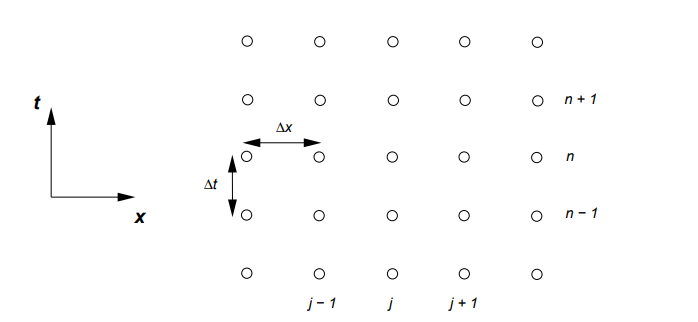
\includegraphics[width = 0.8 \linewidth]{Images/1dPDEwaveFDA_grid.png}
    \caption{Portion of uniform finite-difference mesh (grid) for 1-d time-dependent problem. Note that the spacings in both the spatial and temporal directions are constant}
    \label{fig:enter-label}
\end{figure}

\begin{align}
t^n &\equiv n \Delta t, & n &= 0, 1, 2, \ldots \\
x_j &\equiv (j-1)\Delta x, & j &= 1, 2, \ldots J \\
u_j^n &\equiv u((n-1)\Delta t, (j-1)\Delta x) \\
\Delta x &= (J-1)^{-1} \\
\Delta t &= \lambda \Delta x, & \lambda &\equiv \text{Courant number}
\end{align}

\begin{itemize}
    \item Step 2: Write down FDA for DE (see Figure \ref{fig:FDA_constr})
\end{itemize}

\begin{figure}
    \centering
    
\includegraphics[width = \linewidth]{Images/stencil_PDE_FDA.png}
    \caption{Stencil (molecule/star) for “standard” $O(h^2)$) approximation of (15).}
    \label{fig:FDA_constr}
\end{figure}


\textit{Discretized interior equation}:

\begin{align}
    \frac{u_j^{n+1}-u_j^n}{\Delta t} &= (u_{tt})_j^n + \frac{1}{2} \Delta t (u_{tt})_j^n + O (\Delta t^2) \\
    &= (u_{tt})_j^n + O (\Delta t)
\end{align}

\begin{align}
    \frac{u_{j+1}^n - 2 u_j^n + u_{j-1}^n}{\Delta x^2} &= (u_{xx})^n_j + \frac{1}{12} \Delta x^2 (u_{xxxx})_j^n + O(\Delta x^4)\\
    &= (u_{xx})_j^n + O(\Delta x^2)
\end{align}

FDA

\begin{equation}
    \frac{u_j^{n+1}-u_j^n}{\Delta t} = \sigma \frac{u_{j+1}^n - 2 u_j^n + u_{j-1}^n}{\Delta x^2}
\end{equation}

Where we can view the $u_j^{n+1}$ term as the equation for the unknown.

\begin{itemize}
    \item If we know $u_j^n$ for all j, then can compute $u_j^{n+1}$ for all j (given B.C.'s)
    \item Initialize scheme using

    \[ u_j^1 = u_0(x_j)\]

    where u is the given function

    \item Easy to solve explicitly for $u_j^{n+1} \Rightarrow$ Scheme is called explicit
\end{itemize}

*** Exam Hint Good question *** : 
\begin{itemize}
    \item Be able to discretize all continuum equations that that we use in class (for FDA)
    \item Be able to find the truncation error of these steps
\end{itemize}

Truncation Error
\begin{itemize}
    \item Interior equation

    \[ u_t = \sigma u_{xx} = (\partial_t - \sigma \partial_{xx})u = 0\]

    \item FDA
    \[ \p_t^h -\sigma \p_{xx}^h )u^h = 0 \]

    Where the partial terms in front of the u expression are the L operator and $L^u$ operator as discussed in the truncation section earlier.

    \item Truncation Error

\end{itemize}

\begin{align*}
    \tau ^h &\equiv L^h u \\
    &= (\partial_t^h - \sigma \partial^h_{xx}) u
\end{align*} 

\[ \tau ^h = (\partial_t^h - \sigma \partial^h_{xx}) u = (\partial_t - \sigma \partial_{xx}) u + \ldots \]

where the term in from of u equals to 0 $\Rightarrow$ consistency

\[ \tau^h = \frac{1}{2} \Delta t(u_{tt})^n_j - \frac{1}{12} \sigma \Delta x^2 (u_{xxxx})^n_j + O(\Delta t^2) + O(\Delta x^4)\]

above: Leading order truncation terms

\[ \tau^h= O(\Delta t) + O (\delta x^2) = O(\Delta t, \Delta x^2) \]

above: "First order in time; second order in space"

**"" Guranteed to be on final exam "" ** -Matt \newline

Discretize Boundary Conditions (Homogeneous Dirichlet):

\[ u_1^{n+1} = u_J^{n+1} = 0\]

Discretize Initial Conditions:

\[ u_j^1 = u_0(x_j)\]

Iterative solution procedure

set $u_j^1 \rightarrow u_j^2 \rightarrow u_j^3 \rightarrow \ldots$

Need solution not to blow up (will almost certainly be physical)

\subsection{Stability Analysis}

\begin{itemize}
    \item Heuristic notion of stability: size of numerical solution does not change "too much" as a function of time:

    \begin{equation}
        ||u(t,x)|| \sim  ||u(x,0)||
    \end{equation}

    Where $||\cdot||$ is some suitable norm, such that the $L_2$ norm

    \begin{equation}
        N(t) = ||u(t,x)|| \equiv \left( \int_0^1 u(t,x)^2 dx\right)^{1/2}
    \end{equation}

    \item Write time-dependent FDA in form 

    \[ \mathbf{u}^{n+1} = \mathbf{G}[\mathbf{u}^n],\]

    where $\mathbf{G}$ is some update operator (Matrix), and $\mathbf{u}$ is a column vector.

    \item Can always write FDA in this form by introducing auxiliary variables analogous to what we did for ODEs

    \item Solution at time step n can be written as

    \[ \mathbf{u}^n = \mathbf{G}^{(n-1)} \mathbf{u}^0\]

    \item Now, assume that G matrix has complete set of orthonormal eigenvalues:

    \[ \mathbf{e}_k, \quad k=1,2,\ldots J\]

    and associated eigenvalues 

    \[ \mu_k, \quad k = 1,2,\ldots, J\]

    so that 

    \[ \mathbf{G} \mathbf{e}_k = \mu_k \mathbf{e}_k \qquad k=1,2,\ldots, J\]

    \item Can now decompose initial data (spectral decomposition)

    \[ \mathbf{u}^0 = \sum_{k=1}^J c_k^0 \mathbf{e}_k\]
    \item then 

    \begin{align}
    \mathbf{u}^n &= \mathbf{G}^{n-1} \left(\sum_{k=1}^J c_k^0 \mathbf{e}_k \right) \\
    &= \sum_{k=1}^J c_k^0 (\mu_k)^{n+1} \mathbf{e}_k
    \end{align}

    Where we need the mu term to stay bounded. and the mu term could be complex.
    
    \item Clearly, if the scheme is to be stable, we must have

    \[ |\mu _k| \le 1 \qquad k=1,2, \ldots J\]
\end{itemize}

\begin{figure}
    \centering
    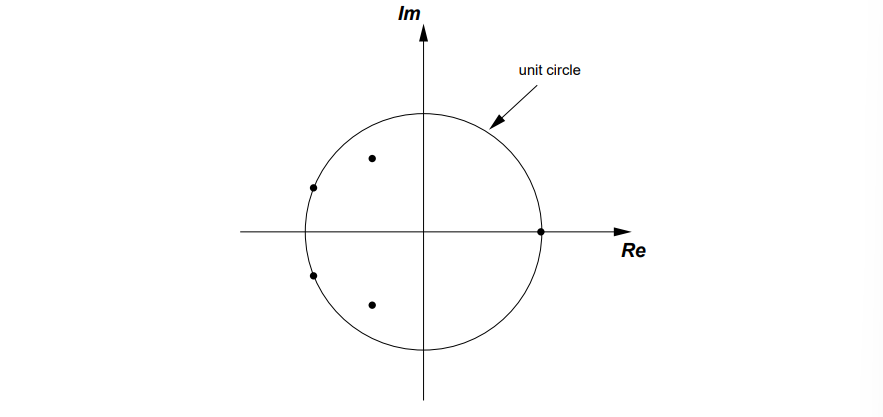
\includegraphics[width = \linewidth]{Images/complex_plane_eigenvalues.png}
    \caption{Schematic illustration of location in complex plane of eigenvalues of update matrix G. In this case, all eigenvalues (dots) lie on or within the unit circle, indicating that the corresponding finite difference scheme is stable.}
    \label{fig:enter-label}
\end{figure}

\subsection{Von-Neumann (Fourier) Stability Analysis}

\begin{itemize}

    \item Von-Neumann stability analysis is based on the ideas sketched in the figure, but additionally assumes
    \begin{itemize}
        \item that the difference equation is linear with constant coefficients,
        \item that the boundary conditions are periodic.
    \end{itemize}

    \item Can use Fourier Analysis: which has the same benefits in the discrete domain -- difference operators in real-space variable x $\rightarrow$ algebraic operations in Fourier-space variable k -- as it does in the continuum 
    
    \item Schematically, instead of 

    \[ \mathbf{u}^{n+1}(x) = \mathbf{G}[\mathbf{u}^n(x)],\]

    \item we consider the Fourier-domain equivalent

    \[ \tilde{\mathbf{u}}^{n+1}(k) = \tilde{\mathbf{G}}[\tilde{\mathbf{u}}^n(x)],\]

    \item where k is the wave number (Fourier-space variable). and the tilde denotes the Fourier transformed version of the different terms.

    \item Define Fourier-transform grid function via

    \begin{equation}
    \tilde{\mathbf{u}}^{n}(k) = \frac{1}{\sqrt{2 \pi}} \int_{\infty}^{\infty} e^{-ikx} \mathbf{u}^n(x) dx
    \end{equation}

    \item For a general difference scheme, we will find that

    \[ \tilde{\mathbf{u}}^{n+1}(k) = \tilde{\mathbf{G}}(\xi)\tilde{\mathbf{u}}^n(k)],\]

    \[ \xi = kh = k \Delta x\]

    Will need to show that $\tilde{\mathbf{G}}(\xi)$'s eigenvalues lie within or on the unit circle for all conceivable $\xi$.

    \item if $\tilde{\mathbf{G}}(\xi)$ is a scalar, then its modulus must be $\le 1$

    \[\tilde{\mathbf{G}}(\xi) \equiv \text{Amplification Matrix / Factor}\]

    \item What is appropriate range for $\xi = kh = k \Delta x$?

    \begin{itemize}
        \item Shortest wavelength representable on uniform mesh with spacing h is $\lambda=2h$ (Nyquist limit), corresponding to a maximum wave number $k = (2\pi )/\lambda = \pm \pi /h$.

        \item Therefore appropriate range is 

        \[ -\pi \le \xi \le \pi, \]
    \end{itemize}
    
    \item Start with VN stability analysis for diffusion equation from last day

    \item Introduce undivided difference operator $D^2$

    \[ D^2 u(x) = u(x+h) - 2u(x) + u(x-h)\]

    \item Supress spatial grid index, differential equation is 

    \[ u^{n+1} = u^n + \alpha D^2 u^n\]
    \[ \alpha = \sigma \frac{\Delta t}{h^2} = \sigma \frac{\Delta t}{\Delta x^2}\]

    \item What's action of $D^2$ in fourier space?

    \item Use inverse F.T.

    \[ u(x) = \frac{1}{\sqrt{2 \pi}} \int_{-\infty}^{\infty} e^{ikx}\tilde{k}dk\]
    so 

    \begin{align}
        D^2 u(x) = u(x + h) - 2u(x) + u(x - h) &= \int_{-\infty}^{\infty} (e^{ikh} - 2 + e^{-ikh})e^{ikx}\tilde{u}(k)dk\\
        &= \int_{-\infty}^{\infty} (e^{i \xi} - 2 + e^{-i\xi}) e^{ikx}\tilde{u}(k)dk
    \end{align}

    \item We can replace the term in brackets with $-4\sin^2(\xi/2)$:

    \[ D^2 u(x) = u(x + h) - 2u(x) + u(x - h) = \int_{-\infty}^{\infty} \left(-4\sin^2(\xi/2)\right)e^{ikx}\tilde{u}(k)dk\]

    \item Missed some points

    \item Amplificaiton Factor in Fourier space:

    \begin{equation}
        \tilde{\mathbf{G}} = 1-4 \alpha \sin^2(\xi/2)
    \end{equation}

    \item Thus, for stability must have

    \[ 4 \alpha \sin^2 (5/2) \le 2 \quad \rightarrow \quad \alpha \le \frac{1}{2}\]

    \begin{equation}
        \alpha = \sigma \frac{\Delta t}{\Delta x^2} \le \frac{1}{2}
    \end{equation}

    \item But of bad news: as $\Delta x \rightarrow 0 , \Delta t$ must $\rightarrow 0$ quadratically in $\Delta x$
    \item In following, will drop integrals, $\frac{1}{\sqrt{2\pi}}$, $e^{ikx}$ and simply write down amplification matrix when it is clear what it is
\end{itemize}

\subsection{Some other discretizations of the diffusion equation}

\subsubsection{Implicit First-Order}

\begin{itemize}
    \item One general way to improve stability of FDAs is to use implicit schemes
    \item Use same mesh, different stencil

    \item FDA

    \[ \frac{u_j^{n+1}-u_j^{n}}{\Delta t} = \sigma \frac{u_{j+1}^{n+1}-2u_j^{n+1}+u_{j-1}^{n+1}}{\Delta x^2}\]

    \item Perform T.S. expansions about $(x_j, t^{n+1})$ get T.E. (verify!)

    \[ \tau = - \frac{1}{2} \Delta t(u_{tt})^{n+1}_{j} + \frac{1}{12} \sigma \Delta x^2 (u_{xxxx})_j^{n+1} + O(\Delta t^2)+ O(\Delta x^2)\]

    \[ \tau = O(\Delta t, \Delta x^2)\]

    First order in time, second order in space

    \item Can't explicitly write down formula for $u_j^{n+1}$ due to coupling of unknowns at $t=t^{n+1}$

    \item Scheme is implicit 

    \item Have to solve (linear) system of equations for $u_j^{n+1}, \qquad j = 1,2,\ldots , J$

    \item Defer solution discussion until stability properties derived

    \item Write scheme as

    \[ u_j^{n+1} = u_j^n + \alpha D^2 u_j^{n+1}\]

    where we are using $\alpha, \quad D$ as previously mentioned

    \[ \Rightarrow (1-\alpha D^2) u^{n+1} - u^n\]

    \item Now apply F.T., get (verify!)

    \[ (1+4\alpha \sin^2 \frac{\xi}{2} \tilde{u}(k)^{n+1} = \tilde{u}(k)^n\]

    \item So, amplification factor is 

    \[ \tilde{G}(\xi) = \frac{1}{1+4\alpha \sin^2\frac{\xi}{2}}\]

    \[ \Rightarrow \tilde{G}(\xi) \le 1 \text{ For ALL } \alpha, \xi\]

    Such a scheme is said to be unconditionally stable (in the VN sense)

    \item VN stability necessary but not necessarily sufficient for "True" stability.

    \textbf{October 30th 2023}

    \item Set $\sigma = 1$ and rearrange earlier equation:
    \[ (-\Delta x^{-2}) u_{j+1}^{n+1} + (\Delta t^{-1} + 2 \Delta x^{-2})u_j^{n+1} +(-\Delta x^{-2})u_{j-1}^{n+1} = (\Delta t^{-1}) u_j^n , \qquad j=2,\ldots, J-1 \]

    \[ u_1^{n+1} = u_J^{n+1} = 0 \qquad \text{(Homogeneous, Dirichlet. B.C.;}\]

    \item In matrix form

    \[ \mathbf{A} \mathbf{u}^{n+1} = \mathbf{b}\]

    What is the structure of matrix A? (non-zero)

    \begin{itemize}
        \item Tri-diagonal system. i.e. three diagonals but everything else is 0.
    \end{itemize}

    \item Special case of \textbf{sparse} matrix, defined as a matrix with a majority of 0 elements (roughly 50 percent or more)

    \item Here, for large J, vast majority of elements will be 0.

    \item Can optimize solution of linear system W.R.T. the sparsity structure

    \item For tridiagonal systems can compute solution in $O(J)$ time vs general $O(J^3)$, BUT have to take advantage of sparsity structure

    \item Recommended approach in MATLAB:

    \begin{verbatim}
        spdiags  % (sparse diagonals)
    \end{verbatim}
    \item Illustrate using example which solves above system ($nx=J$)

    \item Define diagonals of sparse matrix $\mathbf{A}$ as columns of auxiliary matrix $\mathbf{B}$, pass $\mathbf{B}$ along with diagonal numbers to spdiags

    \begin{verbatim}
        % Initialize storage for sparse matrix and RHS

        dl = zeros(nx, 1);
        d = zeros(nx,1);
        du = zeros(nx,1);
        f = zeros(nx,1);

        % Set up tridiagonal system

        dl = -1.0/dx^2 * ones(nx,1);
        d = (1.0/dt * 2.0/dx^2) * ones(nx,1);
        du = dl;

        % Fix up boundary cases

        % Left B.C.
        d(1) = 1.0;
        du(2) = 0.0;

        % Right B.C.
        dl(nx-1) = 0.0;
        d(nx) = 1.0;

        % Define sparse matrix
        % B is [dl d du]
        % -1:1 is which diagonals 
        % nx, nx is dimensions

        A = spdiags([dl d du], -1:1, nx, nx)

        % Define RHS vector 

        f(2:nx-1) = u(n, 2:nx-1)/dt;
        f(1) = 0;
        f(nx) = 0;
    \end{verbatim}

    \item Can then use $\mathbf{A}$ in linear solve via left division

    \begin{verbatim}
        u(n+1,:) = A\f;

        % \ operator knows about sparse matrices; solve is optimized, very fast!
    \end{verbatim}

    \item Can see full matrix (with all 0's included using the full command:

    \begin{verbatim}
        full(A)
    \end{verbatim}

    \item Diagonal in position M from main diagonal has length nx-m
    \item Thus, any column of $\mathbf{B}$ other than the main diagonal will have positions/values that are not used

    \item Diagonal above (super diagonal): At beginning
    \item Diagonal below (sub diagonal): At end

    \item Once more, note how B.C's are implemented

    \[(1)u_1^{n+1} + (0) u_2^{n+1} = 0\]

    \[ (0) u_{J-1}^{n+1} + (1) u_{J}^{n+1} = 0\]
\end{itemize}

\subsubsection{Crank-Nicholson Scheme}

\begin{figure}
    \centering
    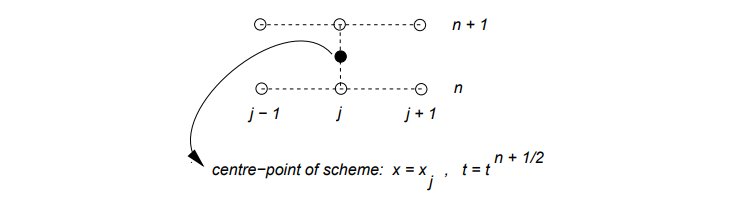
\includegraphics[width = \linewidth]{Images/crank_nicholson_scheme.png}
    \caption{: Stencil (molecule/star) for $O(h^2)$ Crank-Nicholson approximation of (19)}
    \label{fig:crank-nicholson}
\end{figure}

\[ u_t = \sigma u_{xx}\]

Using rectangle stencil with center fictitious point at n+1/2 and j. And that is where you do the taylor series about.

\textbf{FDA}

\begin{equation}
    \frac{u_j^{n+1}-u_j^n}{\Delta t} = \frac{1}{2} \sigma \left[ \frac{u_{j+1}^{n+1} - 2u_j^{n+1} + u_{j-1}^{n+1}}{\Delta x^2} + \frac{u_{j+1}^n-2u_j^n+u_{j-1}^n}{\Delta x^2} \right]
\end{equation}

\textbf{November 1st 2023}

Truncation error takes quite a bit of work; here is the result:

\[ \tau = \frac{1}{24} \Delta t^2 (u_{ttt})_j^{n+\frac{1}{2}} - \frac{1}{8} \sigma \Delta t^2 (u_{ttxx})_j^{n+\frac{1}{2}} - \frac{1}{12} \sigma \Delta x^2 (u_{xxxx})_j^{n+\frac{1}{2}}+O(\Delta t^4) + O(\Delta x^4) + O(\Delta t^2 \Delta x^2)\]

\[ \tau = O(\Delta t^2, \Delta x^2) \Rightarrow \text{ Improved temporal accuracies relative to first two schemes}\]

\begin{itemize}
    \item "Wouldnt ask to derive a truncation error for a scheme like this on the exam but he WOULD ask for us to derive truncation error for previous two schemes"
    \item Make sure you can derive tau for simpler (first order) schemes, ** Exam Hint **
\end{itemize}

Stability
\begin{itemize}
    \item Write scheme
    \[(1- \frac{\alpha}{2} D^2 ) u_j^{n+1} = (1+\frac{\alpha }{2} D^2) u_j^n\]

    $\alpha, \quad D^2$ as previously used
    \item Apply Fourier Transform (get $\rightarrow$ verify)
    
    \[(1+2\alpha \sin^2 \xi/2 ) \tilde{u}(k)^{n+1} = (1-2\alpha \sin^2\xi/2 ) \tilde{u}(k)^n\]
    
    \item Amplification factor is
    \[ \tilde{G}(\xi) = \frac{1-2\alpha \sin^2 \xi/2}{1+2\alpha \sin^2 \xi/2} \]
    \item This is of the form
    \[ \tilde{G}(\xi) = \frac{1-x}{1+x} \qquad x \ge 0 \]

    \[ \tilde{G}(\xi) \le 1 \text{ for all } \xi, \alpha \]

    Scheme is also \textbf{unconditionally} stable

    \item Solution with Crank method yields same structure as the t grid 

    $\Rightarrow$ tridiagonal system

    \item Solve using spdiags as we did for implicit scheme (tutorial next week)
\end{itemize}

\subsubsection{Exact Solution for Testing}

\begin{itemize}
    \item Recall 

    \[ u_t = \sigma u_{xx}\]
    on
    \[ 0 \le x \le 1 \qquad t\ge 0\]

    \[ u(x,0) = u_0(x)\]
    \[u(0,t) = u(1,t) = 0\]

    \item Exact solution

    \[ u(x,t) = e^{-\sigma \omega ^2 t} \sin(\omega t) \]

    where $\omega = n \pi , \qquad n=1,2, \ldots$

    \[ u_t = u_{xx} = -\sigma \omega^2 u(t,x)\]
\end{itemize}


\subsection{The 1-D Schr\"{o}dinger Equation}

\begin{equation}
    i \psi_t = - \frac{\hbar^2}{2m} \psi_{xx} + V(t,x) \psi
\end{equation}

\[ 0 \le x \le 1\]

\[ \psi(t,x) \in \mathbb{C}\]

\[ \text{V(t,x) is given potential} \]

\begin{itemize}
    \item Non-dimensionalize, solve on unit interval with homogeneous Dirichlet B.C.'s 

    \[ i \psi_t = - \psi_{xx} + V \psi \]

    

    \[ \psi(0,x) = \psi_0(x)\]

    \[ \psi(t,0) = \psi(t,1) = 0 \Rightarrow \text{Physical interpretation?}\]

    Infinite potential walls at x=0, 1; no penetration of wave function

    \item Exact solution for testing (V=0)
    \[ \psi(t,x) = e^{i\omega ^2 t } \sin(\omega x)\]

    where $\quad \omega = n \pi , \quad n=1,2,\ldots$

    \textbf{FDA:}

    Use crank-nicholson grid

    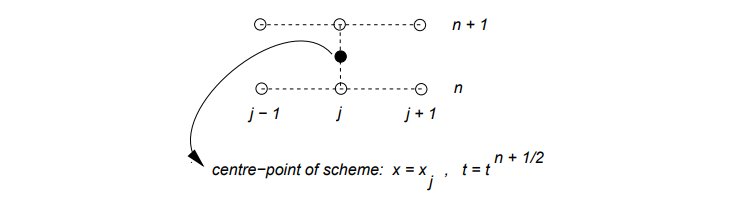
\includegraphics[width =  \linewidth]{Images/crank_nicholson_scheme.png}
    

    \[ \psi_j^{n+\frac{1}{2}} = \frac{1}{2} ( \psi^{n+1}_j + \psi_j^n)\]

    with error of $O(\Delta t^2)$


    \begin{equation}
        i \frac{\psi^{n+1}_j-\psi^n_j}{\Delta t} = -\frac{1}{2}\left( \frac{\psi^{n+1}_{j+1} - 2 \psi_j^{n+1} + \psi _ {j-1}^{n+1}}{\Delta x^2} + \frac{\psi_{j+1}^n-2\psi_j^n + \psi_{j-1}^n}{\Delta x^2}\right) + \frac{1}{2} V_j^{n+\frac{1}{2}} (\psi_j^{n+1}+\psi_j^n) 
    \end{equation}

    \[ \psi^{n+1}_j = \psi^{n+1}_J = 0\]

    \item Truncation error 

    \[ \tau = O(\Delta t^2, \Delta x^2)\]

    Second order in space and time

    \item Stability analysis

    \item \textbf{Theorem}: In stability analysis, can neglect terms that do not include spatial derivatives!

    \item EXAM HINT FOR 830AM final: "undifferentiated terms you don't need to worry about... etc for stability analysis"

    \item Write scheme, without $V \psi$ term, as 

    \[ (i + \frac{1}{2} \alpha D^2) \psi^{n+1} = (i-\frac{1}{2} \alpha D^2) \psi^n\]

    $D^2 $ as before \newline

    $\alpha = \frac{\Delta t}{\Delta x^2}$

    \item Under F.T.

    \[ (i- 2 \alpha \sin^2 \xi/2 ) \tilde{\psi}(k)^{n+1} = (i+2\alpha \sin^2 \xi/2) \tilde{\psi}(k)^n\]
    

    \item Read off amplification factor 

    \[ \tilde{G}(\xi) = \frac{i+2\alpha \sin^2 \xi/2 }{i-2\alpha \sin^2 \xi/2}\]

    Which is of the form

    \[ \frac{1+a}{1-a} \qquad a \text{ REAL}\]
    \[ \left| \frac{i+a}{i-a} \right| = \frac{|i+a|}{|i-a|} = \frac{1+a^2}{1+a^2} = 1\]

    Thus,

    \[ |\tilde{G}(\xi)| = 1 \quad \text{ for all } \xi, \alpha\]

    The scheme is unconditionally stable

    This reflects fact that probability is conserved in the continuum

    "we will see this in play with final project"

    Solution of equations

    \item Rewrite equation as tridiagonal system

    \[ C^+_j \psi_{j+1}^{n+1} + C_j^0 \psi _j^{n+1} + c_j^- \psi_{j-1}^{n+1} = f_j\]

    where only second term of c has actual j dependence from the V psi term

    \item Set up matrix using spdiags, solve using left division (project )
\end{itemize}

\subsection{Wave-equation}

\subsubsection{1-D Wave equation with fixed (dirichlet) B.C.'s}

\[ u_{tt} = u_{xx} \qquad (c=1) \qquad 0 \le x \le 1 \quad t \ge 0\]

\[ u(0,x) = u_0(x)\]

\[ u_t(0,x) = u_0(x)\]

\[ u(t,0) = u(t,1) = 0\]

\begin{itemize}
    \item Step 1: Discretize domain (use same mesh)

    \item Make FDA Characterized by single scale, h

    \[ \Delta t = \lambda \Delta x = \lambda h\]

    \[ h = \Delta x\]

    \[ \lambda = \frac{\Delta t}{\Delta x}\]

    \[ \lambda \equiv \text{"Courant Number"}\]

    \item Whenever we vary $\Delta x$, automatically vary $\Delta t$ ($\lambda$ held constant)

    \item Step 2: Write down FDA:
    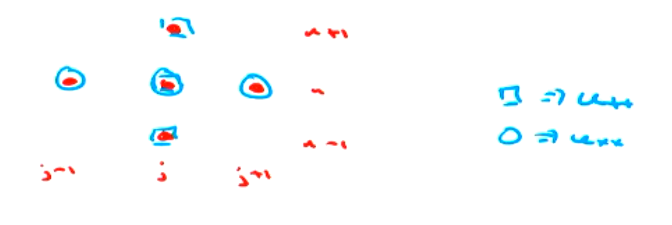
\includegraphics[width = \linewidth]{Images/wave_fda.png}


    MAKE SURE YOU CAN DERIVE THIS FOR EXAM HINT  - if you know the left hand side, also know how to get the expansion on the right hand side***

    
    \[ (\Delta t)^{-2} ( u_j^{n+1}-2u_j^n+u_j^{n-1}) = (u_{tt})_j^n + \frac{1}{12} \Delta t^2 (u_{tttt})_j^n + O(\Delta t^4)\]

    \[ = (u_{tt})_j^n+O(\Delta t^2)\]


    hint: Same expansion (can use similarity argument on exam and not repeat full derivation): 

    
    \[ (\Delta x)^{-2} ( u_{j+1}^{n}-2u_j^n+u_{j-1}^{n}) = (u_{xx})_j^n + \frac{1}{12} \Delta x^2 (u_{xxxx})_j^n + O(\Delta x^4)\]

    \[ = (u_{xx})_j^n+O(\Delta x^2)\]


    \item FDA

    \[ \frac{u_j^{n+1}-2u_j^n+u_j^{n-1}}{\Delta t^2} = \frac{u_{j+1}^n - 2 u_j^n + u_{j-1}^n}{\Delta x^2} \qquad j=2,3,\ldots, J-1\]

    \item Called a ``three level scheme'' since it couples unknowns on 3 time levels 

    \item Truncation error ($\tau = \tau^h = L^h u $; $L^hu^h = 0$)

    First write FDA in form

    \[ \tau = \frac{1}{12} \Delta t^2 (u_{tttt})_j^n - \frac{1}{12}\Delta x^2 (u_{xxxx})_j^n + O(\Delta t^4) + O(\Delta x^4)\]

    \[ = O(\Delta x^2, \Delta t^2) = O(h^2)\]

    Second order in space and time

    \item Discrete B.C.'s 

    \[ u_1^{n+1} = u^{n+1}_J = 0\]

    Missed info 

    \item Discrete I.C.'s

    \begin{itemize}
        \item Need to give two ``time levels" of data (effectively $u(0,x), u_t(0,x)$

        \[ u_j^1 \quad , \quad j=1,2, \ldots , J\]

        \[ u_j^2 \quad , \quad j=1,2, \ldots , J\]
    \end{itemize}

    \item Can solve FDA equation above for $u_j^{n+1}$ explicitly

    \[ u_j^{n+1} = 2u_j^n -u_j^{n-1} + \lambda^2 ( u_{j+1}^n - 2u_j^n + u_{j-1}^n)\]

    \item Initialization revisited 

    \item First time level: $u_0(x)$

    \[ u_j^1 = u_0(x_j)\]

    Second time level: need to determine $u_j^2$ up to and including $O(\Delta t^2)$ terms

    \begin{align}
        u_j^2 &= u_j^1 + \Delta t (u_t)_j^1 + \frac{1}{2} \Delta t^2 (u_{tt})_j^1 + O(\Delta t^3) \\
        &= u_j^1 + \Delta t (u_t)_j^1 + \frac{1}{2} \Delta t^2 (u_{xx})_j^1 + O(\Delta t^3)\\
        &= u_0(x_j) + \Delta t v_0(x_j) + \frac{1}{2} \Delta t^2 u_0''(x_j)
    \end{align}
\end{itemize}

Stability Analysis 
(more involved due to 3 time levels)

\begin{itemize}
    \item Rewrite FDA in ``first order" form by introducing auxiliary variables

    \[ v_j^n = u_j^{n-1} \Rightarrow v_j^{n+1}=u_j^n\]

    \[ \Rightarrow u_j^{n+1} = 2 u_j^n - v_j^n + \lambda^2(u_{j+1}^n - 2u_j^n + u_{j-1}^n)\]

    \[ v_j^{n+1} = u_j^n\]

    \item In matrix form

    \[\begin{bmatrix}
        u \\
        v
    \end{bmatrix}^{n+1} = \begin{bmatrix}
        2+\lambda^2D^2-1 & -1 \\
        1 & 0
    \end{bmatrix}
    \begin{bmatrix}
        {u} \\
        {v}
    \end{bmatrix}^n \]

    Where the D terms is same as $D^2$ previously 
    
    \item Under Fourier Transormation, becomes

    \[\begin{bmatrix}
        \tilde{u} \\
        \tilde{v}
    \end{bmatrix}^{n+1} = \begin{bmatrix}
        2-4\lambda^2 \sin^2 \xi/2 & -1 \\
        1 & 0
    \end{bmatrix}
    \begin{bmatrix}
        \tilde{u} \\
        \tilde{v}
    \end{bmatrix}^n\]

    where the matrix is $\tilde{G}(\xi)$

    \item Need to determine conditions so $\tilde{G}(I)$ has eigenvalues on or within unit circle

    \item Characteristic equation (whose roots are the e.v.'s)

    \[ \begin{vmatrix}
    2-4\lambda^2\sin^2\xi/20-\mu & -1 \\
    1 & \mu
        
    \end{vmatrix} = 0
    \]

    or

    \[ \mu^2 + (4 \lambda^2 \sin^2\xi/2 -2 ) \mu + 1 = 0\]
    Equation has roots at

    \[ \mu ( \xi) = (1-2\lambda^2 \sin^2 \xi/2 ) \pm ((1-2\lambda^2 \sin^2 \xi/2)^2 -1)^{1/2}\]

    Need sufficient conditions for

    \[ |\mu(\xi)| \le 1\]
    Equivalently

    \[ |\mu(\xi)|^2 \le 1\]

    \[ \mu(\xi) = (1-Q) \pm ((1-Q)^2-1)^{1/2} \]

    \[ Q\equiv 2 \lambda^2 \sin^2 \xi/2\]

    \item 3 cases to consider

    \begin{enumerate}
        \item \[(1-Q)^2-1 = 0\]

        \item \[(1-Q^2)-1 < 0\]

        \item \[ (1-Q^2)-1 > 0\]
    \end{enumerate}

    Case 1: $Q=0$ or $Q=2$, In both cases $|\mu(\xi)|=1$

    Case 2: $((1-Q)^2-1)^{1/2}$ purely imaginary

    \[ \mu(\xi) = (1-Q)^2 + (1-(1-Q)^2) = 1\]

    Case 3: $(1-Q)^2 -1 > 0 \rightarrow (1-Q)^2 > 1 \rightarrow Q>2$

    \[ 1-Q - ((1-Q)^2-1) < -1\]

    Instability at
    \[ |\mu(\xi)| > 1\] 

    \item Necessary condition for von Neumann stability

    \[ (1-Q)^2 -1 \le 0 \rightarrow (1-Q)^2 \le 1 \rightarrow Q \le 2\]

    \item But $Q=2\lambda^2 \sin^2 \xi/2 \quad ; \quad 2 \lambda^2 \le 2 ; \quad \lambda^2 \le 1$

    For stability we need
    \[ \lambda \equiv \frac{\Delta t}{\Delta x} \le 1\]

    \item This condition is often called the CFL condition—after Courant, Friedrichs and Lewy who derived it in 1928 (the ratio $\lambda = \Delta x/ \Delta t$ is also frequently called the \textit{Courant number}). In practical terms, we must limit the time-discretization scale , $\Delta t$, to values no larger than the space-discretization scale, $\Delta x$. Furthermore, this type of instability has a “physical” interpretation, often summarized by the statement \textit{the numerical domain of dependence of an explicit difference scheme must contain the physical domain of dependence}.

    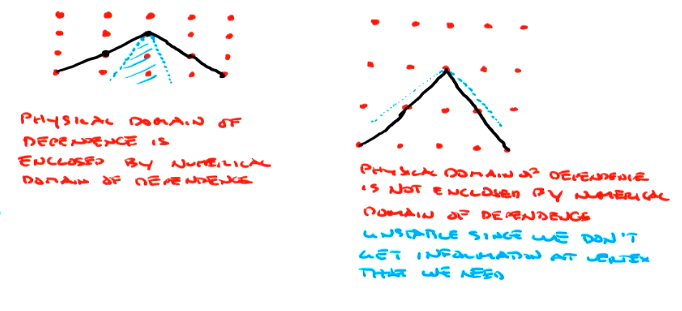
\includegraphics[width = 0.9 \linewidth]{Images/CFL_condition.png}

    \item EXAM HINT : make sure you can do a stability analysis like this!! Really good exam question

\end{itemize}

\textbf{November 6th 11:19am}

\subsection{Dispersion in FDAs}

\begin{itemize}
    \item Advection Equation

    \[ u_{t} = a u_x\]

    \item Exact solution

    \[u(t,x) = f(at+x)\]

    Propogates initial data profile to the left with speed a. No change in profile's shape $\Rightarrow$ non-dispersive. Every fourier component travels with the same speed c.

    \item Semi-discretization: only discretize in space

    \[ u_t = a D_x u = a \frac{u_{j+1}-u_{j-1}}{2\Delta x}\]
    Leave time continuous

    \item Look for normal mode solutions, of the form

    \[ u = e^{ik(x+G't)}\]

    $k \equiv $ to the wave number \newline
    $a' \equiv $ to the discrete phase speed associated with k

    \item Substitute in (a')

    \[ ika' u = \frac{a (2 i \sin(k \Delta ))}{2\Delta x} u \]

    \item Solve for a'

    \[ a' = a \frac{\sin(k \Delta x)}{k\Delta x} = a \frac{\sin\xi}{\xi}\]

    \[ \xi \equiv k \Delta x\]

    \item Low frequency limit $\xi \rightarrow 0$

    \[ a' = \lim_{\xi\rightarrow0} a \frac{\sin\xi}{\xi} = a \]

    Expected result

    \item High frequency limit, $\xi \rightarrow \pi$

    \[ a' = a \frac{\sin \pi}{\pi} = 0 \]

    Highest frequency components don't propagate at all

    \item Typically of low-order FDAs

    \item In practice may want to damp high-frequency components by adding explicit dissipation to the scheme

    \item High-frequency components often responsible for instabilities
\end{itemize}

End of discussion about PDEs in 1-D